In Fig. \ref{fig:2.2.4_quadrilateral},

\begin{align}
\vec P - \vec S &= \myvec{3 +2\\0+1}
= \myvec{5\\1}
\\
\vec Q - \vec P &= \myvec{4-3\\5-0}
= \myvec{1\\5}
\end{align}
Thus, the area of the rhombus can be calculated as 
\begin{align}
\norm{ \mathbf{\left(\vec P - \vec S\right)} \times \mathbf{\left(\vec Q - \vec P\right)}}
&= \norm{ \mathbf{\myvec{5\\1}} \times \mathbf{\myvec{1\\5}}}
	\\
	\norm{\Delta} = 5 \times 5 - 1 \times 1&= 24
\end{align}
\begin{figure}[!ht]
	\centering
	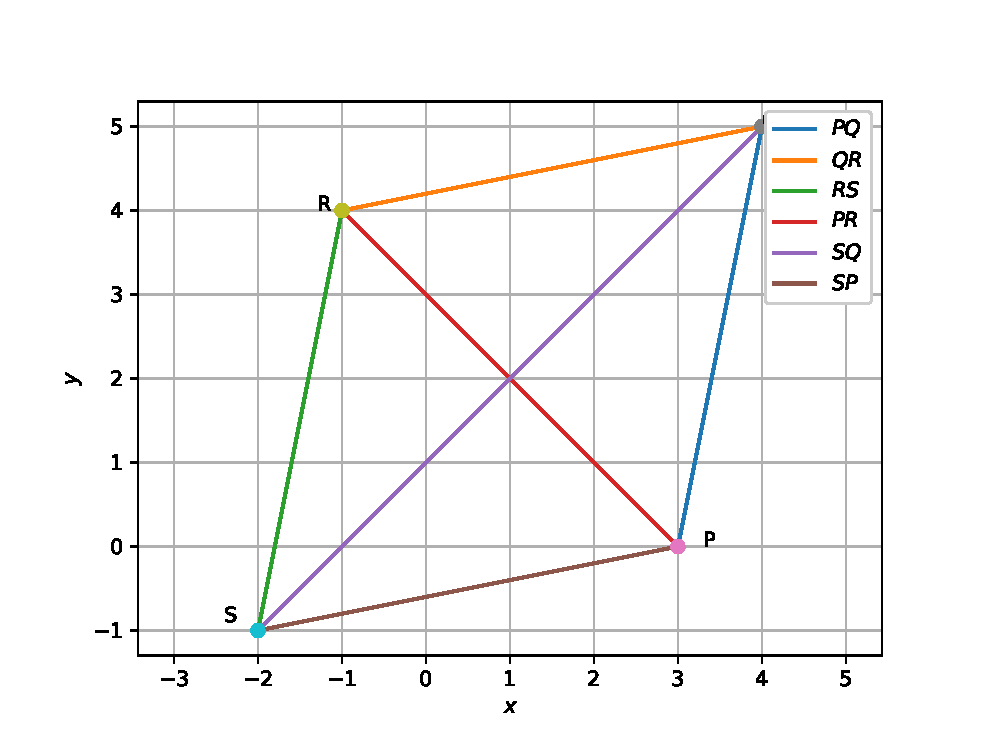
\includegraphics[width=\columnwidth]{./solutions/4/figures/quadrilateral/quad.eps}
	\caption{}
	\label{fig:2.2.4_quadrilateral}
\end{figure}
\begin{lstlisting}
solutions/4/codes/quadrilateral/quad.py
\end{lstlisting}


